\documentclass[border=1pt]{standalone}
\usepackage[T1]{fontenc}\usepackage{helvet}\renewcommand{\familydefault}{\sfdefault}
\usepackage{tikz}\usetikzlibrary{arrows.meta}
\definecolor{ink}{HTML}{1B2733}\definecolor{boxc}{HTML}{E4E9EF}
\definecolor{gr}{HTML}{DDEFDD}\definecolor{grt}{HTML}{235C30}
\definecolor{am}{HTML}{F8EBCF}\definecolor{amt}{HTML}{7A4C08}
\definecolor{rd}{HTML}{F7DFDF}\definecolor{rdt}{HTML}{862424}
\newcommand{\solved}{\tikz[baseline=-.6ex]\fill (0,0) circle (1.9pt);}
\newcommand{\partf}{\tikz[baseline=-.6ex]{\fill[sharp corners] (0pt,-1.8pt) arc[start angle=-90,end angle=90,radius=1.8pt] -- cycle;\draw[line width=.5pt] (0pt,0pt) circle[radius=1.8pt];}}
\newcommand{\open}{\tikz[baseline=-.6ex]\draw[line width=.5pt] (0,0) circle (1.8pt);}
\newcommand{\sw}[1]{\tikz[baseline=-.7ex]\fill[#1,rounded corners=1pt] (0,-2.8pt) rectangle (9pt,2.8pt);}
\newcommand{\nohy}{\hyphenpenalty=10000 \exhyphenpenalty=10000 }
% \pill{style}{x}{y}{width}{label}{text}{status icon}
\newcommand{\pill}[7]{%
  \node[#1,minimum width=#4,text width=#4-15pt] (q) at (#2,#3) {\textbf{#5}\ #6};
  \node[anchor=east,inner sep=0pt,text=ink] at ([xshift=-3.5pt]q.east) {#7};}
\begin{document}
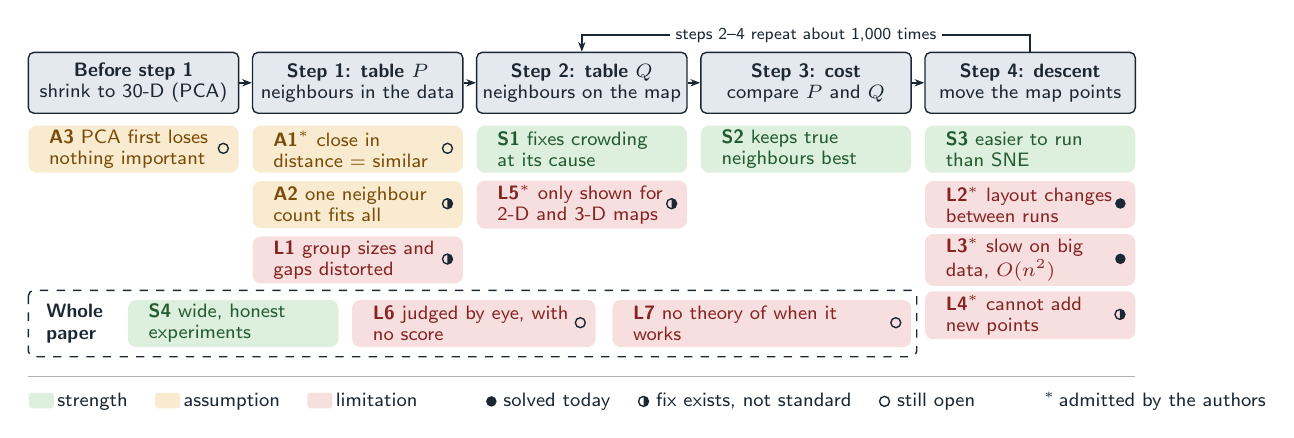
\begin{tikzpicture}[x=1pt,y=1pt,
 st/.style={draw=ink,line width=.5pt,rounded corners=2pt,fill=boxc,minimum width=76pt,minimum height=22pt,inner sep=1pt,align=center,text=ink,font=\fontsize{7}{8}\selectfont},
 p/.style={rounded corners=3pt,minimum height=17pt,inner xsep=3pt,inner ysep=1.5pt,align=left,font=\fontsize{6.7}{7.6}\selectfont\nohy},
 S/.style={p,fill=gr,text=grt},A/.style={p,fill=am,text=amt},L/.style={p,fill=rd,text=rdt},
 ar/.style={-{Stealth[length=3.5pt]},draw=ink,line width=.6pt}]
\foreach \i/\a/\b in {0/Before step 1/shrink to 30-D (PCA),1/Step 1: table $P$/neighbours in the data,2/Step 2: table $Q$/neighbours on the map,3/Step 3: cost/compare $P$ and $Q$,4/Step 4: descent/move the map points}
  \node[st] (s\i) at (\i*81,0) {\textbf{\a}\\[-.5pt]\b};
\foreach \i/\j in {0/1,1/2,2/3,3/4} \draw[ar] (s\i)--(s\j);
\draw[ar] (s4.north) -- ++(0,6) -| node[pos=.25,fill=white,inner xsep=2pt,inner ysep=0pt,font=\fontsize{6.2}{7}\selectfont,text=ink]{steps 2--4 repeat about 1{,}000 times} (s2.north);
% pills under the step that causes them
\pill{A}{0}{-24}{76pt}{A3}{PCA first loses nothing important}{\open}
\pill{A}{81}{-24}{76pt}{A1$^*$}{close in distance = similar}{\open}
\pill{A}{81}{-44}{76pt}{A2}{one neighbour count fits all}{\partf}
\pill{L}{81}{-64}{76pt}{L1}{group sizes and gaps distorted}{\partf}
\pill{S}{162}{-24}{76pt}{S1}{fixes crowding at its cause}{}
\pill{L}{162}{-44}{76pt}{L5$^*$}{only shown for 2-D and 3-D maps}{\partf}
\pill{S}{243}{-24}{76pt}{S2}{keeps true neighbours best}{}
\pill{S}{324}{-24}{76pt}{S3}{easier to run than SNE}{}
\pill{L}{324}{-44}{76pt}{L2$^*$}{layout changes between runs}{\solved}
\pill{L}{324}{-64}{76pt}{L3$^*$}{slow on big data, $O(n^2)$}{\solved}
\pill{L}{324}{-84}{76pt}{L4$^*$}{cannot add new points}{\partf}
% whole paper
\draw[draw=ink,dashed,line width=.5pt,rounded corners=2pt] (-38,-75) rectangle (283,-99);
\node[anchor=west,align=left,font=\fontsize{7}{8}\selectfont,text=ink] at (-35,-87) {\textbf{Whole}\\\textbf{paper}};
\pill{S}{36}{-87}{76pt}{S4}{wide, honest experiments}{}
\pill{L}{123}{-87}{88pt}{L6}{judged by eye, with no score}{\open}
\pill{L}{227}{-87}{108pt}{L7}{no theory of when it works}{\open}
% legend, outside the grid
\draw[ink!35,line width=.4pt] (-38,-106) -- (362,-106);
\node[anchor=west,inner sep=0pt,text=ink,font=\fontsize{6.7}{8}\selectfont] at (-38,-115)
 {\sw{gr}\,strength \quad \sw{am}\,assumption \quad \sw{rd}\,limitation
  \qquad\quad \solved\ solved today \quad \partf\ fix exists, not standard \quad \open\ still open
  \qquad\quad $^*$\,admitted by the authors};
\end{tikzpicture}
\end{document}
